\section{Hooke's law}
\label{sec:hooke}

\subsection*{Comment}

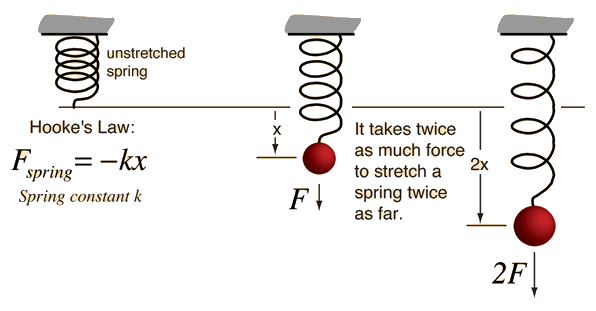
\includegraphics[scale=0.5]{hook.png}\\
\emph{(\href{http://hyperphysics.phy-astr.gsu.edu/hbase/imgmec/hook.gif}{Image} from HyperPhysics by Rod Nave, Georgia State University)}

Second-order differential equations deal with oscillations. Here we consider harmonic oscillation of a spring. The aim of this challenge is to give you the opportunity to think about how the terms of a 2nd-order ODE relate to force and stiffness in the context of a spring.

Equation \ref{eq:hooke} is a fundamental equation of mechanics describing oscillatory motion such as the spring here. Hooke's law states that the force leading to acceleration of the mass $m$ is proportional to the stretching distance $x$. The proportionality constant is Hooke's constant, $k$.

\begin{equation}
    \label{eq:hooke}
    m x'' + k x = 0
\end{equation}
or alternatively
\begin{equation}
    \label{eq:hooke2}
    m x'' = -k x
\end{equation}

This leads to perfectly oscillating motion,
\begin{equation}
    \label{eq:oscillation}
     x(t)=\cos(\omega t)
\end{equation}
which oscillates forever since there is no damping term.

\subsection*{Challenge}
By considering the oscillatory motion (equation \ref{eq:oscillation}) as a solution of the 2nd-order differential equation given by Hooke's law (equations \ref{eq:hooke} and \ref{eq:hooke2}), determine the oscillation frequency $\omega$ in terms of the mass and spring constant.

\subsection*{Solution}
To check your answer, calculate the oscillation frequency for a harmonic spring with a mass of \SI{2}{kg} and spring-constant of \SI{4}{kg/s^2}. Only enter numbers, without any units, in your answer.

\soltwodp{g}{9553fe}




%%%%%%%%%%%%%%%%%%%%%%%%%%%%%%%%%
\newpage
%%%%%%%%%%%%%%%%%%%%%%%%%%%%%%%%%
\section{Exponentials and trigonometry}

\subsection*{Resources}
\begin{itemize}
    \item Text: \url{https://www.phy.duke.edu/~rgb/Class/phy51/phy51/node15.html}
\end{itemize}

\subsection*{Challenge}
Write $\sin(x)$ and $\cos(x)$ in exponential form.

\subsection*{Solution}
Please compare your solution with your partner or discuss with the teacher.




%%%%%%%%%%%%%%%%%%%%%%%%%%%%%%%%%
\newpage
%%%%%%%%%%%%%%%%%%%%%%%%%%%%%%%%%
\section{Characteristic equation: understanding}

\subsection*{Resources}
\begin{itemize}
    \item Book (\url{http://tutorial.math.lamar.edu/getfile.aspx?file=B,1,N}) from page 106.
\end{itemize}

\subsection*{Comment}
It is possible to add a damping term $B$ to Hooke's law that is proportional to the velocity of the movement. You could imagine this as a friction term, with the force from friction becoming stronger as the velocity increases.

\subsection*{Challenge}
\begin{equation}
    A \frac{d^2y}{dt^2} + B \frac{dy}{dt} + C y = 0
\end{equation}

Show that, assuming that all solutions to a 2nd-order differential equation of the form above will have solutions $y(t)=e^{rt}$, the value of $r$ can in principle be determined by solving the following a quadratic equation of the form
\begin{equation}
    A r^2 + Br + C = 0
\end{equation}

\subsection*{Solution}
If you are unsure of your derivation, please ask someone.




%%%%%%%%%%%%%%%%%%%%%%%%%%%%%%%%%
\newpage
%%%%%%%%%%%%%%%%%%%%%%%%%%%%%%%%%
\section{Characteristic equation: roots}

\subsection*{Resources}
\begin{itemize}
    \item Book (\url{http://tutorial.math.lamar.edu/getfile.aspx?file=B,1,N}) from page 106.
\end{itemize}

\subsection*{Challenge}
Sum the points of the differential equations that have characteristic equations with
\begin{itemize}
    \item Real, distinct roots
    \item Complex roots
    \item Equal roots
\end{itemize}

1 point: $\displaystyle -3 y'' - 5 y' + 2 y = 0$ % C

2 points: $\displaystyle 3 y'' - 4 y' + 3 y = 0$ % E

4 points: $\displaystyle 3 y'' - 6 y' + 3 y = 0$ % B

8 points: $\displaystyle 3 y'' - 5 y' + 2 y = 0$ % F

16 points: $\displaystyle 3 y'' - 5 y' + 4 y = 0$ % D

32 points: $\displaystyle 3 y'' + 5 y' + 2 y = 0$ % A

\subsection*{Solution}

\subsubsection*{Real, distinct roots}
\solint{i}{dc6ada}

\subsubsection*{Complex roots}
\solint{j}{7c030b}

\subsubsection{Equal roots}
\solint{k}{c90b44}




%%%%%%%%%%%%%%%%%%%%%%%%%%%%%%%%%
\newpage
%%%%%%%%%%%%%%%%%%%%%%%%%%%%%%%%%
\section{Characteristic equation: real roots with positive B}

\subsection*{Resources}
\begin{itemize}
    \item Book (\url{http://tutorial.math.lamar.edu/getfile.aspx?file=B,1,N}) from page 108.
\end{itemize}

\subsection*{Challenge}
1. Solve the following 2nd-order differential equation that has real roots:

\begin{equation}
    \label{eq:ccrrpb}
    y'' + 3 y' + 2 y = 0
\end{equation}

2. What is the effect of including a positive damping (friction) term?

\subsection*{Solution}
1. $y(1) = 1.14$ given initial conditions $y(0)=5$ and $y'(0)=-8$.

2. Please compare your answer with your partner or discuss with the teacher in class.




%%%%%%%%%%%%%%%%%%%%%%%%%%%%%%%%%
\newpage
%%%%%%%%%%%%%%%%%%%%%%%%%%%%%%%%%
\section{Characteristic equation: real roots with negative B}

\subsection*{Resources}
\begin{itemize}
    \item Book (\url{http://tutorial.math.lamar.edu/getfile.aspx?file=B,1,N}) from page 108.
\end{itemize}

\subsection*{Comment}
Here we include a damping term again, but this time it is positive.

\subsection*{Challenge}
1. Solve the following 2nd-order differential equation that has real roots. 

\begin{equation}
    y'' - 3 y' + 2 y = 0
\end{equation}

2. What is the effect of changing the damping term from positive to negative?

\subsection*{Solution}
1. $y(1) = -47.13$ given initial conditions $y(0)=5$ and $y'(0)=-8$.

2. Please compare your answer with your partner or discuss with the teacher in class.




%%%%%%%%%%%%%%%%%%%%%%%%%%%%%%%%%
\newpage
%%%%%%%%%%%%%%%%%%%%%%%%%%%%%%%%%
\section{Characteristic equation: B in equations with real roots}

\subsection*{Challenge}

\emph{(Note that there are two parts to this challenge.)}

Considering the equation

\begin{equation}
    A y'' + B y' + C y = 0
\end{equation}

1 point: Positive damping (positive B) leads to solutions with exponentials with positive exponents.

2 points: Positive damping (positive B) leads to solutions with exponentials with negative exponents.

4 points: Negative damping (negative B) leads to solutions with exponentials with positive exponents.

8 points: Negative damping (negative B) leads to solutions with exponentials with negative exponents.

16 points: Exponentials with positive exponents (eg, $e^{t}$) lead to exponential growth (instability).

32 points: Exponentials with negative exponents (eg, $e^{-t}$) lead to exponential growth (instability).

64 points: Exponentials with positive exponents (eg, $e^{t}$) lead to a damped signal (stability).

128 points: Exponentials with negative exponents (eg, $e^{-t}$) lead to a damped signal (stability).

\subsection*{Solution}
\solint{o}{8e808b}



\iffalse
%%%%%%%%%%%%%%%%%%%%%%%%%%%%%%%%%
\newpage
%%%%%%%%%%%%%%%%%%%%%%%%%%%%%%%%%
\section{Characteristic equation: equal roots}

\subsection*{Resources}
\begin{itemize}
    \item Book (\url{http://tutorial.math.lamar.edu/getfile.aspx?file=B,1,N}) from page 117.
\end{itemize}

\subsection*{Comment}
It is not necessary to follow the full derivation in the suggested resource.

\subsection*{Challenge}
Solve the equation
\begin{equation}
    y'' - 2y' + y = 0
\end{equation}
subject to the initial conditions $y(0)=5$ and $y'(0)=6$.

\subsection*{Solution}
$y(1)=16.310$




%%%%%%%%%%%%%%%%%%%%%%%%%%%%%%%%%
\newpage
%%%%%%%%%%%%%%%%%%%%%%%%%%%%%%%%%
\section{Characteristic equation: complex roots with B=0}

\subsection*{Resources}
\begin{itemize}
    \item Book (\url{http://tutorial.math.lamar.edu/getfile.aspx?file=B,1,N}) from page 112.
\end{itemize}

\subsection*{Challenge}
1. Assuming there is no damping term (ie, $B=0$) show that the roots for the differential equation
\begin{equation}
    A y'' + Cy = 0
\end{equation}
are $\pm i \sqrt{C/A}$.

2. Solve the following ODE:
\begin{equation}
    \label{eq:cecr}
    y'' + 4 \pi^2 y = 0
\end{equation}
subject to the initial conditions $y(0)=4$ and $y'(0)=10 \pi$.

\subsection*{Solution}
$y(0.4)=-0.297$




%%%%%%%%%%%%%%%%%%%%%%%%%%%%%%%%%
\newpage
%%%%%%%%%%%%%%%%%%%%%%%%%%%%%%%%%
\section{Characteristic equation: complex roots with positive B}

\subsection*{Resources}
\begin{itemize}
    \item Book (\url{http://tutorial.math.lamar.edu/getfile.aspx?file=B,1,N}) from page 112.
\end{itemize}

\subsection*{Challenge}
Solve the following ODE:
\begin{equation}
    y'' + y' + y = 0
\end{equation}
subject to initial conditions $y(0)=8$ and $y'(0)=2$. One of the integration constants is $4 \sqrt{3}$. You will need to find the other one.

\subsection*{Solution}
$y(0.4)=8.0867$




%%%%%%%%%%%%%%%%%%%%%%%%%%%%%%%%%
\newpage
%%%%%%%%%%%%%%%%%%%%%%%%%%%%%%%%%
\section{Characteristic equation: complex roots with negative B}

\subsection*{Resources}
\begin{itemize}
    \item Book (\url{http://tutorial.math.lamar.edu/getfile.aspx?file=B,1,N}) from page 112.
\end{itemize}

\subsection*{Challenge}
Solve the following ODE:
\begin{equation}
    y'' - y' + y = 0
\end{equation}
subject to initial conditions $y(0)=1$ and $y'(0)=2$. One of the integration constants is $\sqrt{3}$. You will need to find the other one.

\subsection*{Solution}
$y(0.4)=1.867$




%%%%%%%%%%%%%%%%%%%%%%%%%%%%%%%%%
\newpage
%%%%%%%%%%%%%%%%%%%%%%%%%%%%%%%%%
\section{Damping}
\label{sec:damping}

\subsection*{Resources}
\begin{itemize}
    \item Wikipedia: \url{https://en.wikipedia.org/wiki/Damping}
\end{itemize}

\subsection*{Challenge}
Of the 6 functions shown in the graph, place the 3 that correspond to over-damped, critically damped and under-damped in the order mentioned in this sentence.

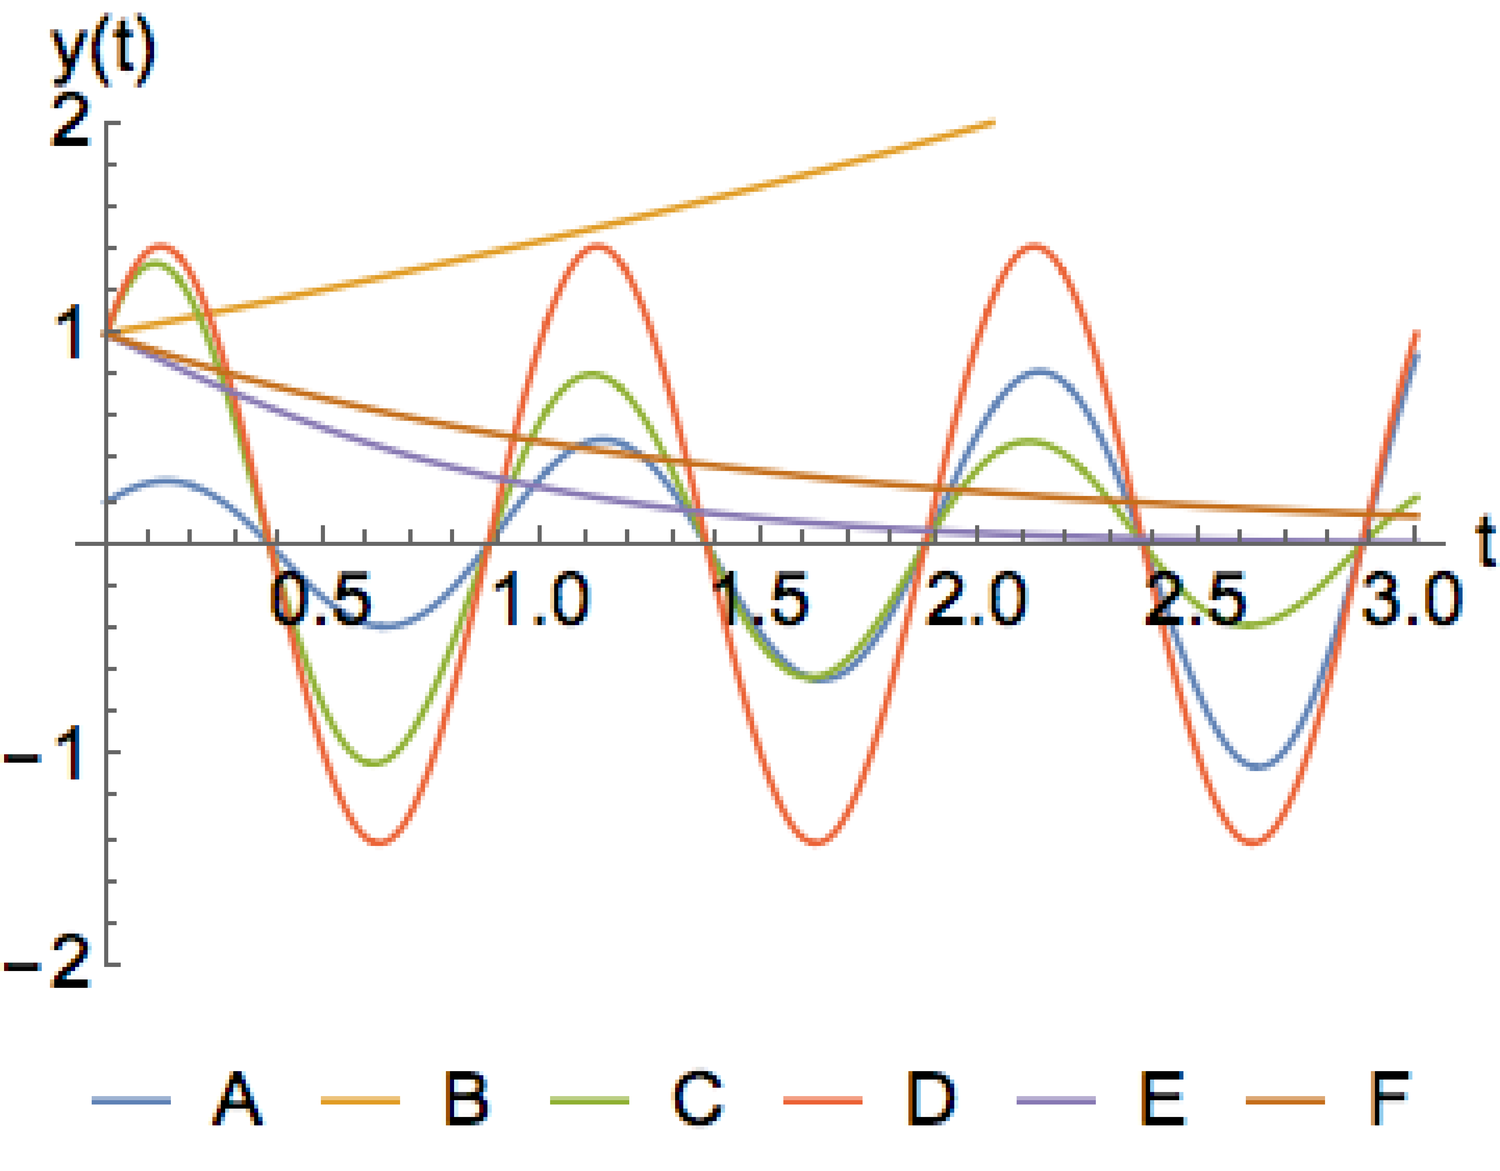
\includegraphics[scale=0.75]{damping.png}
\subsection*{Solution}
(eg, ``abc'')

\solstr{t}{b3f888}




%%%%%%%%%%%%%%%%%%%%%%%%%%%%%%%%%
\newpage
%%%%%%%%%%%%%%%%%%%%%%%%%%%%%%%%%
\section{Damping and 2nd-order differential equations} % NT: Restore impossible solution part, keeping C>0, A>0 too.

\subsection*{Challenge}
1. The 6 functions shown in the graph in challenge \ref{sec:damping} may represent solutions of a 2nd-order differential equation $Ay'' + By' + C = 0$. Assuming $A>0$ and $C>0$, place the solutions A-F in the order shown below.% Note that one of the descriptions below is impossible, and you should ignore that one.

I. Solution of a 2nd-order differential equation with real roots and positive B.

II. Solution of a 2nd-order differential equation with real roots and negative B.

III. Solution of a 2nd-order differential equation with equal roots.

IV. Solution of a 2nd-order differential equation with complex roots and B=0.

V. Solution of a 2nd-order differential equation with complex roots and positive B.

VI. Solution of a 2nd-order differential equation with complex roots and negative B.

\subsection*{Solution}
(eg, ``abcdef'')

\solstr{u}{33db25}




%%%%%%%%%%%%%%%%%%%%%%%%%%%%%%%%%%
%\newpage
%%%%%%%%%%%%%%%%%%%%%%%%%%%%%%%%%%
%\section{The Wronskian}
%
%\subsection*{Resources}
%\begin{itemize}
    %\item Book (\url{http://tutorial.math.lamar.edu/getfile.aspx?file=B,1,N}) from page 125 and page 130.
%\end{itemize}
%
%\subsection*{Challenge}
%
%\emph{Please write the following answers clearly and in a manner that can be easily shared with others in the class.}
%
%1. What is meant by a ``fundamental set of solutions''?
%
%2. Why is the final solution for real and complex roots always a sum of two terms?
%
%3. What is the ``Wronskian'', and what is the formula for its calculation?
%
%4. Considering $C_1 y_1(t) + C_2 y_2(t) = 0$, how is linear dependence and independence defined?
%
%5. How can the Wronskian be used to determine linear independence?
%
%\subsection*{Solution}
%Please read at least 1 other peer's solution and discuss any differences. The teacher will also help check your understanding.




%%%%%%%%%%%%%%%%%%%%%%%%%%%%%%%%
\newpage
%%%%%%%%%%%%%%%%%%%%%%%%%%%%%%%%
\section{Characteristic equation: exercises}

\emph{(Note that if you encounter a square-root during your calculations such as $\sqrt{7}$, it is best to work with $\sqrt{7}$ rather than $2.65$ in order to maintain accuracy until the final step where you need to evaluate it. If the equation becomes too messy (eg $e^{(\sqrt{7}-1)/\sqrt{3}}$) you can always substitute $m=(\sqrt{7}-1)/\sqrt{3}$, etc, to make things clearer.)}

\subsection*{Challenge}
1. Determine $y(1)$ for the equation

\begin{equation}
    2 y''+8y'+y=0    
\end{equation}
given the initial conditions $y(0)=4$ and $y'(0)=3$.

2. Determine $y(0.2)$ for the equation

\begin{equation}
    2y''+4y'+2y=0
\end{equation}
given the initial conditions $y(0)=4$ and $y'(0)=2$.

3. Determine $y(0.1)$ for the equation

\begin{equation}
    4y''+3y'+y=0
\end{equation}
given the initial conditions $y(0)=6$ and $y'(0)=2$.


\subsection*{Solution}
1. 4.32 %\hash{vv}{f01192}

2. 4.26 %\hash{ww}{6f5d64}

3. 6.19 %\hash{xx}{c74f58}




%%%%%%%%%%%%%%%%%%%%%%%%%%%%%%%%
\newpage
%%%%%%%%%%%%%%%%%%%%%%%%%%%%%%%%
\section{Non-homogeneous equations: Method of undetermined coefficients}

\subsection*{Resources}
\begin{itemize}
    \item Video: All 4 Khan Academy videos starting at \url{https://www.khanacademy.org/math/differential-equations/second-order-differential-equations/undetermined-coefficients/v/undetermined-coefficients-1}
    \item PDF: \url{http://www.math.psu.edu/tseng/class/Math251/Notes-2nd\%20order\%20ODE\%20pt2.pdf}
\end{itemize}

\subsection*{Comment}
The 2nd-order equations we were considering until now were homogeneous equations (ie, the RHS was zero). We can now build upon this to expand our ability to solve non-homogeneous equations (ie, where the RHS of the equation is non-zero).

The Khan Academy videos give an excellent initial introduction to the subject, and so please do take the time to view and take notes about all four videos in the series. The PDF listed above then allows us to develop our repertoire much further and explains very clearly about cases more-complicated than the videos. Please therefore make notes covering the material in the PDF from page 11 to onwards. Prior pages are largely covered by the videos.

You may note that in the PDF, the particular solution is denoted by $Y$ while Sal Khan denotes it as $y_p$ in the videos.

\subsection*{Challenge}
Complete questions 1-4 on page 22 in the PDF. These first challenges cover the fundamental basic cases upon which all subsequent cases are built.

\subsection*{Solution}
The questions in this challenge are taken from the PDF and the answers can be found on the last page. Perhaps obviously, since you will not have the answers in a real-life/exam environment, please don't review each answer until completion. If you get stuck, be sure to review your notes (especially the worked-examples in the PDF) rather than the answers, to facilitate deep learning. 




%%%%%%%%%%%%%%%%%%%%%%%%%%%%%%%%
\newpage
%%%%%%%%%%%%%%%%%%%%%%%%%%%%%%%%
\section{Method of undetermined coefficients II}

\subsection*{Resources}
\begin{itemize}
    \item PDF: \url{http://www.math.psu.edu/tseng/class/Math251/Notes-2nd\%20order\%20ODE\%20pt2.pdf}
\end{itemize}

\subsection*{Challenge}
Continuing from the previous challenge, complete questions 5-10 on page 22 in the PDF. For at least 1 of these, make up some initial conditions (eg, $y(0)=1$, $y'(0)=2$) and try to solve for those conditions. These challenges introduce a range of more complex situations and thus provide excellent practise of the concepts covered. 

\subsection*{Solution}
The questions in this challenge are taken from the PDF and the answers can be found on the last page. Perhaps obviously, since you will not have the answers in a real-life/exam environment, please don't review each answer until completion. If you get stuck, be sure to review your notes (especially the worked-examples in the PDF) rather than the answers, to facilitate deep learning. 




%%%%%%%%%%%%%%%%%%%%%%%%%%%%%%%%
\newpage
%%%%%%%%%%%%%%%%%%%%%%%%%%%%%%%%
\section{Method of undetermined coefficients III}

\subsection*{Resources}
\begin{itemize}
    \item PDF: \url{http://www.math.psu.edu/tseng/class/Math251/Notes-2nd\%20order\%20ODE\%20pt2.pdf}
\end{itemize}

\subsection*{Comment}
This challenge gives you useful practise of going the other way; determining a differential equation that describes a given solution. This can be a little confusing at first, so take time to understand where things originate from.

\subsection*{Challenge}
Complete challenges 19 and 20 from page 23 of the PDF.

\subsection*{Solution}
The questions in this challenge are taken from the PDF and the answers can be found on the last page. Perhaps obviously, since you will not have the answers in a real-life/exam environment, please don't review each answer until completion. If you get stuck, be sure to review your notes (especially the worked-examples in the PDF) rather than the answers, to facilitate deep learning. 



\fi
